\section{Pipeline di baking}
\label{sec:chapter_baking_service_pipeline_baking}
L’operazione di Bake, in questo lavoro di tesi, avviene tramite l’utilizzo di un processo Blender installato su un server remoto. Blender in questo lavoro di tesi ha permesso la creazione e l’applicazione di texture lightmap sugli oggetti presenti nella scena creata in Three.js.
\\
Questa procedura risulta però complessa da effettuare in quanto prevede una profonda conoscenza, da parte di chi la utilizza, dell’algoritmo di bake e dei parametri che esso accetta. Inoltre è necessaria una buona esperienza nell’utilizzo di Blender, un software difficile da padroneggiare.
\\
Nel dettaglio per permettere a Blender la creazione delle lightmap, la scena creata in ambiente web (descritta tramite il formato JSON4) deve essere importata, tale e quale a quella originale, all’interno del software Blender. 
\\
Questa importazione all’interno di un linguaggio differente, quello Python, risulta un’operazione complessa.
\\
Una volta che la scena è stata importata correttamente in Blender, verranno calcolate ed applicate le informazioni di luce (lightmap) agli oggetti inseriti. 
Infine la scena, con applicate le informazioni di luce, verrà esportata nel file di scambio JSON 4. All’interno di quest’ultimo vengono infatti trascritte tutte le strutture dati Python in un formato comprensibile a Three.js.
\\
L’obiettivo principale di questo lavoro è stato quindi quello di automatizzare il processo di creazione delle lightmap al fine di semplificare l’esperienza dell’utente che utilizza questo sistema. 
\\
L’utente infatti una volta creata la scena in Three.js dove solamente premere un pulsante ed il processo di bake penserà ad effettuare tutte le elaborazione in maniera totalmente autonoma.
\\
L’elaborazione risulta quindi completamente trasparente e l’utilizzatore non si accorge del fatto che il flusso di dati in input (il json creato in Three.js) deve passare attraverso più passi di elaborazione (una pipeline quindi).
L’implementazione di ognuno di questi passi è stata realizzata tramite il linguaggio Python, sfruttando le API fornite da Blender.
In particolare nel presente lavoro è stato creato uno script bake.py che permettesse di svolgere questi passi in maniera totalmente automatica.
\\
I passi da effettuare sono:
\begin{itemize}
\item Il caricamento all’interno di Blender della scena Three.js ricevuta come input tramite il formato JSON4. Prevede la creazione di un parser scritto in Python.
\item Il mapping tra il rendering Rasterization di Three.js con il rendering Path Tracing (Cycles render) di Blender.
\item Il ciclo di bake durante il quale vengono calcolate ed applicate le lightmap.
\item L’esportazione della scena da Blender nel linguaggio Three.js tramite la scrittura di un file JSON4.
\end{itemize}

Il caricamento della scena prevede l’analisi del file in entrata al fine di riconoscere le strutture dati Three.js ed adattarle in quelle utilizzate dalle API di Blender.
Questo adattamento è specifico per le due tecnologie utilizzate ed è ugualmente valido per entrambi i render di Blender: Blender render e Cycles render.
\\
Il mapping risulta un’operazione complessa in quanto ha il compito di mappare specificatamente un rendering di tipo rasterization in un rendering di tipo path tracing (chiamato Cycles render in Blender).
Questo tipo di mappatura è stato oggetto di studio e sperimentazioni in questo lavoro di tesi in quanto non esiste una metodologia standard che permettesse di effettuarla. Questa operazione in particolare viene dettagliata nel paragrafo \ref{sec:chapter_baking_service_pipeline_baking_mapp_parametri}.
\\
Anche l’operazione di bake è stata studiata approfonditamente al fine di comprendere come Blender la effettuasse. Sono state effettuate sperimentazioni tramite l’interfaccia grafica fornita dal software al fine di comprendere quali parametri influenzassero il Bake e quali valori assegnare ad essi per ottenere i risultati voluti. L’operazione di bake è stata poi replicata tramite codice sfruttando le API messe a disposizione da Blender.
\\
Il ciclo di bake viene effettuato grazie all’utilizzo di CUDA, l'architettura di elaborazione in parallelo di NVIDIA. 
CUDA ha infatti permesso, in questo lavoro di tesi, miglioramenti netti nei tempi di bake rispetto a computazioni basate su CPU grazie allo sfruttamento della potenza di calcolo delle GPU (unità di elaborazione grafica).
\\
Per l’esportazione è stato utilizzato come base un addon (scritto in Python) già esistente, descritto in \cite{io_three} , che permettesse di effettuare questa operazione. Esso però risultava incompleto in quanto non permetteva la scrittura di alcune strutture dati fondamentali. Le modifiche apportate all’ exporter verrano approfondite nel paragrafo \ref{sec:chapter_baking_service_pipeline_baking_esport_scena}.
\\
Realizzare lo script è risultata quindi un’operazione complessa in quanto ha reso necessario un accurato studio delle strutture dati utilizzate da Three.js e dalle API di Blender.
Inoltre è stato effettuato un accurato lavoro di ricerca su come effettuare il mapping tra due rendering differenti, anch’ essi studiati dettagliatamente.
\\
Questa fase di studio e sperimentazione è stata velocizzata grazie all’utilizzo del Node Editor, fornito da Blender.
Il suo utilizzo permette una metodologia di programmazione molto potente e flessibile che sfrutta i nodi al fine di modificare i materiali degli oggetti, le texture ed il rendering in generale.
\\
Esso è stato sfruttato principalmente durante la fase di mapping, come spiegato nel paragrafo \ref{sec:chapter_baking_service_pipeline_baking_mapp_parametri}, ed ha permesso di riprodurre alcuni materiali tipici di un Rasterization render tramite la creazioni di complessi materiali in Blender.
\\
Inoltre durante la realizzazione dello script sono state utilizzate due differenti modalità che hanno permesso di lavorare in maniera differente con gli oggetti geometrici:
\begin{itemize}
\item \texttt{Object Mode}: permette di effettuare le operazioni che influenzano l’intero oggetto come ad esempio la traslazione, rotazione la scalatura.
\item \texttt{Edit Mode}: permette di effettuare le operazioni che agiscono sulla geometria dell’oggetto, ma non sulle proprietà globali. Ad esempio permette la modifica dei vertici della geometria.
\end{itemize}
Le due modalità inoltre utilizzano strutture dati differenti, non è però compito di questo elaborato trattare le differenze.
Salvo dove diversamente specificato in questo capitolo si assume che le operazioni vengano effettuate in modalità Object Mode. 


\subsection{Caricamento della scena}
\label{sec:chapter_baking_service_pipeline_baking_caricam_scena}
Il caricamento della scena è il primo passo di elaborazione effettuato dallo script installato in Blender. Questo processo risulta avviato su un server remoto che, tra le varie funzioni, intercetta le richieste effettuate dal client (l’editor).
\\
Nella richiesta viene inviato il file .json che rappresenta la scena 3D in Three.js descritta tramite le strutture dati ed i parametri previsti dal rendering di tipo Rasterization.
Questo file viene poi analizzato dallo script creato nel presente lavoro di tesi per permettergli di effettuare il caricamento della scena.
\\
L’analisi prevede in particolare il riconoscimento  delle informazioni Three.js riportate sul json al fine di adattarle in strutture dati utilizzate in Blender.
\\
Di fatto la scena Three.js descritta nel JSON4 viene analizzata, mediante un algoritmo ricorsivo, a partire dall’ oggetto JSON che rappresenta la scena, per definizione il padre di ogni oggetto presente.
\\
Ogni oggetto descritto nel formato JSON viene quindi riconosciuto ed adattato nella struttura dati corrispondente In Blender. Quest’ultimo espone infatti una API scritta in Python per la creazione di scene 3D, molto differente dal linguaggio Three.js.
\\
Viene ora presentato una pseudocodifica dei passi effettuati dall’analizzatore:
\\
\begin{algorithm}
	json = load\_json (json\_path);\hspace{5pt}add\_object(Empty)\;
	\For{ogni json\_ob nella scena, visitata in profondità}{
	    \If{has\_geo(json\_ob)}{
			json\_geometry=take\_geo\_fromJson(json\_ob)\;
	    	json\_material=take\_mat\_fromJson(json\_ob)\;
	    	verts=take\_verts(json\_geometry);\hspace{5pt}faces=calculate\_faces()\;
			mesh=new mesh(verts, faces);\hspace{5pt}object=new object (mesh)\;
	    	\If{json\_material}{
	        mat=\textbf{mappingMateriale(json\_material)}\;
	        object.active\_material=mat\;
	        }
	        \If{has\_normal(json\_geometry)}{
	        add\_normal(object,geometry)\;
	        }
	        \If{has\_texture(json\_material)}{
	    	apply\_texture(object,json\_material)\;
	    	apply\_uv(object,json\_geometry)\;
	    	}
		}
	    \If{is\_light(json\_ob)}{
	    	light\_type=json\_ob.type;\hspace{5pt}object=\textbf{mappingLuce(json\_ob)}\;
	    }
		\If{is\_ob3D(json\_ob)}{
	    	ob=Empty;\;
	    }
		apply\_transformations(ob, getMatrix(json\_ob))\;
		\If{has\_parent(json\_ob)}{
	    	json\_parent=parent(json\_ob);\hspace{5pt}ob.parent=json\_parent\;
	    	}
		add\_object(ob)\;
	}
\end{algorithm}
\\
La scena descritta nel json viene visitata tramite una visita in profondità ricorsiva. 
Questo permette di riportare in Blender la medisima gerarchia della scena creata in Three.js.
Per ogni oggetto json individuato vengono effettuate delle operazioni di adattamento che permettono di creare in Blender le corrispondenti strutture dati Three.js.
\\
Alcune delle operazione di adattamento sono indicate all’interno della pseudocodifica riportata, altre sono invece incapsulate all’interno dei metodi riportati che, per semplifità di descrizione dell’importer, sono stati descritti solamente mediante la loro interfaccia.
\\
L’oggetto scena scritto nel JSON, rappresentato  tramite un Object3D, viene prima individuato dall’importer e poi  adattato ad una struttura dati che in Blender viene chiamata Empty. 
Come visibile nella pseudo, questo oggetto Empty viene aggiunto, all’inizio del caricamento, come padre della nuova scena che verrà creata in Blender.
\\
Questo tipo di adattamento Object3D-Empty avviene inoltre per ogni Object3D individuato dall’importer.
\\
Le due strutture dati risultano analoghe in quanto rappresentano un oggetto vuoto (null) e non contengono una vera geometria o materiale. Sia gli Object3D che gli Empty vengono normalmente assegnati come padri di un certo numero di oggetti ai quale si vuole che subiscano le medesime trasformazioni effettuate sul padre. Quindi se un oggetto A è padre di un oggetto B e viene applicata una trasformazione ad A, la medesima trasformazione viene applicata anche su B.
\\
Fortunatamente sia Three.js che Blender trattano la gerarchia della scena in maniera equivalente. Quindi essa non ha avuto bisogno di adattamenti ma è stata riportata esattamente come viene descritta nel formato di scambio Three.js.
\\
Successivamente per ogni oggetto 3D descritto nel file JSON in entrata viene valutato se esso:
\begin{itemize}
\item contiene una geometria (e quindi vertici) e cioè se esso rappresenta effettivamente un oggetto solido 3D.
\item rappresenta una luce, essa verrà quindi mappata in una luce Blender secondo il meccanismo spiegato nel paragrafo \ref{sec:chapter_baking_service_pipeline_baking_mapp_parametri} e quindi aggiunta nella scena Blender.
\item rappresenta un Object 3D e quindi non ha assegnato una geometria, come spiegato precedentemente verrà adattato ad un oggetto Empty di Blender e poi aggiunto nella scena.
\end{itemize}
Per creare un oggetto 3D in Blender è necessario prima creare una mesh, cioè una collezione di vertici (verts), spigoli (edges) e facce (faces) che definiscono la forma dell’ oggetto da rappresentare, e poi creare l’oggetto vero e proprio da aggiungere alla scena. Questo oggetto di solito include la mesh, il materiale e le texture appplicate al materiale.
\\
In Blender la funzione \texttt{from\_pydata} che permette di creare la mesh, accetta come parametri le informazioni dei vertici, degli spigoli e delle facce. Queste tre informazioni sono assegnate alla mesh ed inserite all’interno dei 3 array corrispondenti.
\\
Nel formato JSON4 di Three.js però sono solamente inserite le informazioni dei vertici, scritte all’interno di un array. L’ informazioni delle facce, come spiegato nel paragrafo \ref{sec:formato_scambio_formato_json4}, è ridondante in quanto i vertici dei triangoli vengono scritti nel formato di scambio secondo l’ordine di renderizzazione. Inoltre esattamente come Three.js la primitiva base utilizzata nel rendering sono i triangoli e non i quadrati, quindi ogni faccia è costituita solamente da tre vertici. 
Questo permette di rappresentare l’informazione delle facce tramite un array bidimensionale così costituito: [[0,1,2],[3,4,5],[6,7,8],[9,10,11],…,[n-2,n-1,n]].
\\
Ogni valore dell’array bidimensionale rappresenta infatti un triangolo ed ogni valore del triangolo rappresenta un indice che permette l’individuzione del vertice (x,y,z) all’interno dell’array dei vertici della mesh creata in Blender tramite la funzione \texttt{from\_pydata}.
\\
Infine l’informazione degli spigoli viene omessa in quanto totalmente ridondante per via della presenza delle facce. 
Gli spigoli di solito vengono utilizzati per la creazione di oggetti senza facce. Essi però risultano totalmente inutili in questo lavoro di tesi in quanto permettono di ottenere oggetti costituiti solamente da lati che di fatto nel mondo reale non esistono.
\\
\begin{figure}[htb]
 \centering
 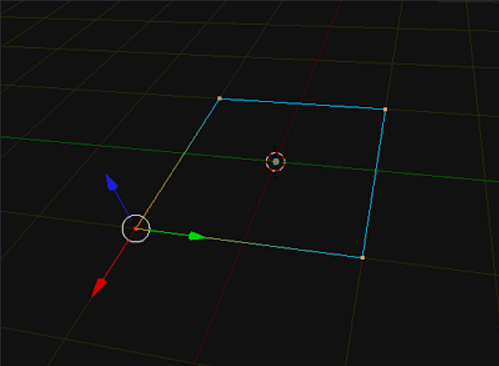
\includegraphics[width=0.6\linewidth]{images/chapter_baking_service/Blender_spigoli.png}\hfill
 \caption[Blender e gli spigoli]{Un oggetto senza facce in Blender}
 \label{fig:baking_service_Blender_spigoli}
\end{figure}


Quindi una volta creata la mesh è possibile creare l’object 3D che rappresenta l’oggetto vero e proprio all’interno della scena. Operazioni quali ad esempio creazione e modifica dei materiali, l’assegnazione di texture e le trasformazioni possono essere effettuate solamente sull’ oggetto.
\\
Il materiale associato all’oggetto nel JSON, quindi proveniente dal render Three.js, non può essere assegnato al nuovo oggetto creato in Blender perchè quest’ultimo utilizza un render differente. 
\\
Questi due render utilizzano infatti tipologie di materiali differenti e per questo è necessario convertire un materiale Three.js in un materiale Cycles render (Blender). Questa operazione risulta molto complessa e verrà spiegata nel paragrafo \ref{sec:chapter_baking_service_pipeline_baking_mapp_parametri}.
\\
Inoltre se nell’oggetto json sono descritte anche le normali ad esso associate, queste verranno prelevate ed assegnate all’oggetto creato in Blender.
\\
In questo lavoro di tesi viene supposto infatti che le normali scritte nel json, e quindi quelle create ad hoc per l’oggetto, risultino quelle ideali per l’oggetto e quindi migliori di quelle che riuscirebbe a creare Blender.
Supposizione che poi si è rivelata veritiera in fase di sperimentazione.
\\
Utilizzando le normali di vertici originali è possibile ottenere l’effetto \emph{smooth shading} desiderato, invece utilizzando le normali calcolate da Blender si ottiene un \emph{flat shading} (\ref{fig:baking_service_flat_smooth}).
Nello smooth shading le normali memorizzate per ogni vertice vengono interpolate, questo permette di non osservare la forma delle facce di cui è costituito dell’oggetto.
\\
\begin{figure}[htb]
 \centering
 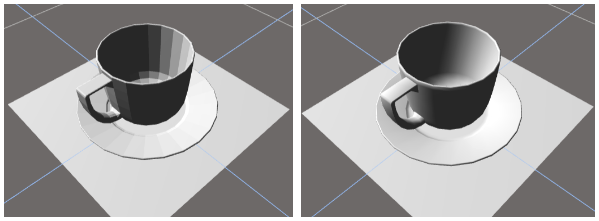
\includegraphics[width=1\linewidth]{images/chapter_baking_service/flat_smooth.png}\hfill
 \caption[Smooth shading e flat shading in Blender.]{A sinistra un effetto smooth shading, a destra un  effetto flat shading}
 \label{fig:baking_service_flat_smooth}
\end{figure}
In Blender, esattamente come Three.js, di default le normali sono uscenti dal lato frontale della faccia (\emph{front\_side}) di ogni geometria. 
Ci sono casi in cui si rende necessario però utilizzare oggetti Three.js con le normali uscenti dalla faccia anteriore (\emph{back\_side}).
\\
\begin{figure}[htb]
 \centering
 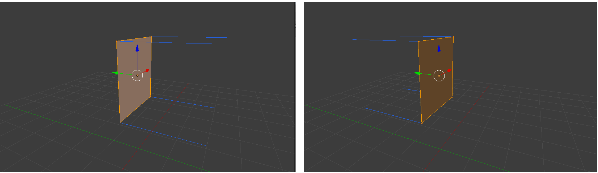
\includegraphics[width=1\linewidth]{images/chapter_baking_service/front_back_side.png}\hfill
 \caption[Front side e back side in Blender.]{A sinistra normali front side, a destra normali back side}
 \label{fig:baking_service_front_back_side}
\end{figure}
Blender tramite l’utilizzo della funzione \texttt{flip\_normals()} permette di girare le normali front\_side e di assegnarle alla faccia opposta, permettendo in questo modo di ottenere le normali back\_side (figura: \ref{fig:baking_service_front_back_side}. 
\\
Adattare correttamente le normali è stato importante in quanto esse sono fondamentali per il corretto calcolo delle luci e per la corretta creazione delle lightmap.
La lightmap viene calcolata sul lato frontale della faccia se le normali sono front\_side, altrimenti sul lato opposto se sono back\_side.
\\
Purtroppo però inserire queste normali non è una operazione semplice in quanto Blender ricalcola automaticamente le normali ogni volta che dalla modalità \emph{object} si passa alla modalità \emph{edit}, sovrascrivendo quelle vecchie.
\\
In particolare il passaggio alla modalità edit in questo lavoro si rende necessario per effettuare il flip delle normali e per effettuare il baking.
\\
Di fatto attualmente non esiste un modo per evitare questa sovrascrittura delle normali. L’unica possibilità per evitarla è salvare localmente in una struttura dati l’associazione geometria e normali importate. Questa struttura dati viene sfruttata prima di effettuare l’esportazione della scena, descritta in \ref{sec:chapter_baking_service_pipeline_baking_esport_scena}, per forzare l’inserimento delle normali originali nelle geometrie degli oggetti.
Come spiegato in precedenza l’utilizzo delle normali create da Blender deve essere assolutamente evitato per impedire l’esportazione da Blender verso Three.js di una scena in cui gli oggetti che sarebbero dovuti essere smooth sono in realtà flat.
\\
Se all’ oggetto json è assegnata una diffuse texture allora la stessa deve essere applicata al corrispondente oggetto Blender. L’assegnazione della texture all’oggetto non è un’operazione semplice. 
Viene prelevato dal json la stringa che rappresenta l’immagine codificata in base 64. Questa viene poi decodificata, convertita nella texture corrispondente e memorizzata da Blender.
\\
Per assegnare la texture all’oggetto Blender è necessario aggiungere al suo materiale un \texttt{texture\_slot} che ha il compito di memorizzare la texture assegnata. 
A questo punto la texture viene memorizzata nello slot associato all’oggetto.
\\
Per poter associare le coordinate uv (inserite in un array) alla texture è necessario prima inserirle all’interno di una struttura dati della mesh chiamata \texttt{uv\_layer}.
\\
Ad ogni uv\_layer, in cui sono inserite le coordinate uv, è necessario assegnare un nome che risulta fondamentale al fine di identificarlo.
Nel presente lavoro di tesi sono stati creati per ogni mesh due differenti uv\_layer (con associati nomi differenti), uno per la diffuse\_map e l’altro per la lightmap.
\\
Entrambi gli uv\_layer hanno assegnate le stesse coordinate uv, questo per permettere la creazione di una lightmap perfettamente coincidente alla diffusemap (a meno delle informazioni di luce) per permette l’ottenimento dei vantaggi descritti nel paragrafo \ref{sec:chapter_lrl_li_te_ba}.
\\
Infine alla diffuse texture ed alla lightmap vengono assegnate le corrispondenti uv (le stesse nel nostro lavoro).
Durante il caricamento della scena, nessuna lightmap viene creata, quindi l’uniche uv considerate sono quelle riguardanti la diffuse texture.
\\
Il motivo per cui vengono utilizzati due uv\_layer verrà dettagliato durante il paragrafo \ref{sec:chapter_baking_service_pipeline_baking_ciclo_bake}.
\\
Per ogni texture è inoltre necessario necessario effettuare una mappatura del parametro repeat ed una mappatura del colore da assegnare al materiale, diverso se possiede la texture o meno. Questa mappatura verrà descritta nel capitolo x.

Una volta applicata la texture vengono eseguite le trasformazioni di traslazione, rotazione e scalatura all’oggetto creato.
Nel json tutte le trasformazioni da applicare all’oggetto sono riportate in una matrice di trasformazione associata all’oggetto JSON. In figura \ref{fig:baking_service_matrix} è rapprentata una matrice di trasformazione; non è però compito di questa elaborato spiegarne il funzionamento.
\\
\begin{figure}[htb]
 \centering
 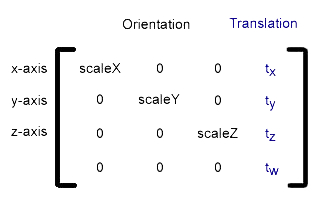
\includegraphics[width=0.6\linewidth]{images/chapter_baking_service/matrix.jpg}\hfill
 \caption[Matrice di trasformazione]{Una matrice di trasformazione.}
 \label{fig:baking_service_matrix}
\end{figure}

Tramite l’utilizzo di una libreria Blender chiamata trasformation.py è stato possibile ottenere queste informazioni dalla matrice di trasformazione. 
In particolare la funzione utilizzata è chiamata decompose() che accetta come parametro la matrice scritta come lista (lista identica a quella presente nel JSON) e permette di ottenere come risultato le tre trasformazioni.
\\
Le informazioni di traslazione e scalatura possono essere applicate direttamente così come sono sugli oggetti Blender. 
Purtroppo questo non è però possibile per la rotazione in quanto la funzione produce come risultato un quaternione. Il quaternione deve essere infatti prima convertito in un angolo di eulero per potere poi essere applicato sull’oggetto.
Anche questa conversione è stata possibile grazie ad una funzione della libreria \texttt{transformation.py}.
Infine l’oggetto viene aggiunto alla scena Blender, pronto per subire l’operazione di bake.

